% sections/measurement.tex -- Section 4, measuring the pipeline without a human reference (five subsections).
% Rewritten 2026-11-21 by the section writer of the PaperOrchestra-style rewrite (outline.json, section_plan).
% Integrator's page cut (2026-11-21): the writer's cuts (c) and (d), the triangle bound to Appendix A (which states it
%   in full), shorter wording throughout; every remaining claim keeps its caveat.
% Every number is a macro of findings/*.tex or floats/caption-notes.tex; floats are generated and only \input here.
% Literal numerals are design constants: 30-s windows, the 15-s shift, 0.25-s, 1-s and 3-s bins, 0.3-s pauses,
%   5 to 60 minutes, 6 min, 0.1 and 0.2 SD, 20% and 10% (injection grid and median), ranks 1--5 and 6--20,
%   the 5-creator rule, 10th and 90th percentiles.
% Floats placed here: fig:seams (figure*, 4.2). tab:anchors and fig:coverage moved to Appendix A (A.2, A.5) by the
%   integrator's page cut; 4.1 and 4.4 refer to them.

\section{Measuring the pipeline without a human reference}
\label{sec:measure}

Every number here from text, segments, word times or the voice detector comes from seen creators (the census of
Section~\ref{sec:coverage} counts all creators' recordings); all are exploratory (registry amendment A2), not tests of
registered hypotheses. The creator is the unit: intervals resample creators or are $t$ intervals on creator values,
95\% unless marked 90\%. Agreement between machines is never accuracy. Appendix~\ref{app:measure} gives each estimand
and weighting.

\subsection{Agreement anchors}
\label{sec:anchors}

Table~\ref{tab:anchors} (Appendix~\ref{app:measure}) gives the ladder of anchors, each a comparison of two machines on
its own scale. With no reference known to be made by people, the usual check against human text
\cite{proksch2019testing} is not run; anchors on possibly human-made texts of non-seen creators are not yet produced
(Appendix~\ref{app:protocol}).

On \AnchorCaptionRecordings{} seen recordings, one per creator (about \AnchorCaptionWords{} caption words), a re-decode
with the run's settings differs from platform automatic captions on \AnchorCaptionMeanPct\% of caption words (creator
mean; $t$ \AnchorCaptionMeanTLo--\AnchorCaptionMeanTHi), \AnchorCaptionPooledPct\% pooled. The captions are machine
text too, and these recordings, set aside before the run at the newest listing ranks (Section~\ref{sec:coverage}), are
no sample of the run. The normaliser, chosen after the first result, lower-cases, drops fillers and expands
contractions, so this anchor is blind to case, filler and contraction errors.

The run's code reproduces the same recognizer's earlier text exactly in \AnchorReproExact{} of
\AnchorReproRecordings{} recordings; the others differ for a reason the materials do not record. A larger model's
earlier text differs by \AnchorLargerModelPct\% (\AnchorLargerModelCreators{} creators; rough, added after the plan).
Without the captions' own error rate, these disagreements bound nothing about the run's error
(Appendix~\ref{app:measure}).

\paragraph{Two recognizer models on the same audio.}
\label{sec:bridge}
In the bridge, both models transcribed English recordings of 5 to 60 minutes, one per creator (\BridgePairs{} registered pairs, all
but fewer than 5 from seen creators; filter version 1). Against a margin of \BridgeMargin{} between-creator SD (SD of
creator means) fixed in advance, \BridgeAgree{} of \BridgeMeasures{} measures agree on average on \BridgeSeenPairs{}
seen pairs, \BridgeDiffer{} differ and \BridgeOpen{} are not settled (90\% intervals; within-creator scale
\BridgeAgreeWithin, \BridgeDifferWithin, \BridgeOpenWithin; Table~\ref{tab:bridge-verdicts}). Pace, pronoun and
contraction rates, word length and word variety agree; word duration, pauses, words per segment and filled pauses
differ; the artefact measures and mean word probability are not settled. As both models see the same detector-gated audio, agreement on pace may
be partly mechanical. The median pair disagrees on \BridgeDisagreeMedianPct\% of words (quartiles
\BridgeDisagreeQOnePct\% and \BridgeDisagreeQThreePct\%; filter version 2). Across models, only agreeing word measures
may be compared, on average and descriptively.

\subsection{Window seams and the grid shift}
\label{sec:seams}

\begin{figure*}[t]
\centering
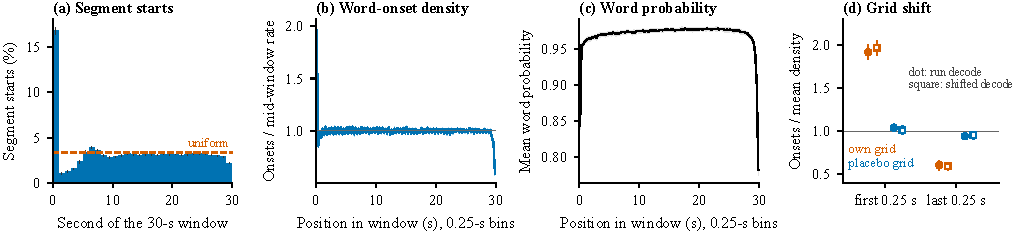
\includegraphics[width=\textwidth]{floats/fig_seams.pdf}
\caption{The fixed 30-s decoding grid marks the transcripts. \CapSeams{} Filter off in (a) to (c). In (d) each decode
is read on its own grid and on the other grid (placebo); dot: run decode, square: shifted decode. No audio was played.}
\label{fig:seams}
\end{figure*}

\SegStartSecZeroPct\% of segments start in a window's first second (uniform: \UniformSecondPct\% per second;
Figure~\ref{fig:seams}). Word onsets in the first 0.25\,s are \OnsetFirstQuarter{} times the mid-window rate, at word
probability \WordProbFirstQuarter; in the last 0.25\,s, \OnsetLastQuarter{} times, at \WordProbLastQuarter. Word times
are the recognizer's, not forced-aligned: \ZeroGapPct\% of within-segment gaps
are zero, and \PauseAtBoundaryPct\% of pauses of 0.3\,s or more sit at segment boundaries. The grid makes
\GridPauseSurplusPct\% of gaps of 0.3 to 30\,s (gaps pooled; 90\% \GridPauseSurplusLo--\GridPauseSurplusHi), \GridPauseTimePct\% of pause time, and
\GridFillerLastThreePct\% of filled pauses in a window's last 3\,s above the flat rate (90\%
\GridFillerLastThreeLo--\GridFillerLastThreeHi).

\paragraph{Grid shift.} \GsRecordings{} seen recordings, one per creator, were decoded again on a grid moved by 15\,s.
Decoding is deterministic: all \GsControlIdentical{} re-decodes on the run grid reproduce the record. The shift changes
\GsChangedPct\% of words (\GsChangedLo--\GsChangedHi; worker versions do not inflate this, Appendix~\ref{app:measure}).
\GsEditsNearRunSeamPct\% of edits lie within 1\,s of a run-grid seam, about \GsNearSeamRatio{} times the uniform
\GsUniformNearSeamPct\%, though most lie elsewhere. In a negative control \cite{lipsitch2010negative}, onset density in
a window's first 0.25\,s is \GsOnsetFirstOwn{} times the mean on a decode's own grid but \GsOnsetFirstPlacebo{} on the
other grid (Figure~\ref{fig:seams}d): the shift separates seam effects on onsets and timing from the speech.

The pause share moves by \GsPauseShareSd{} between-creator SD (\GsPauseShareSdLo{} to \GsPauseShareSdHi) and word
counts by \GsWordsDiffPct\%. On average no pause measure moves by more than \GsPauseSdMax{} SD and no word measure by
more than \GsWordSdMax{} SD, filled pauses excepted (\GsFillerSd; \GsFillerSdLo{} to \GsFillerSdHi;
Table~\ref{tab:gridshift}); these are intervals, not equivalence tests, on a lenient yardstick for change within one
recording. As no word crosses its own seam, own seams fall in pauses more often than placebo seams
(\GsSeamInPauseOwnPct\% against \GsSeamInPausePlaceboPct\%), so the seam rule's assumption of gaps independent of grid
phase (Section~\ref{sec:pipeline}) fails in part. The rule keeps creators' rank order (rank correlation at least
\SeamRuleRankCorrMin), so pause results are within-model rankings, not levels; timing measures are whole-span rates,
and thanks-phrase counts are tied to one grid position.

\subsection{An apparently inserted phrase and the positional filter}
\label{sec:artefacts}

Whisper-family models write fluent phrases with no speech behind them, tied to non-speech audio or long non-vocal
stretches \cite{koenecke2024careless,baranski2025investigation}. Here a stand-alone two-word thanks phrase, a closing
courtesy, appears to be inserted at window ends. On the run grid it starts in a window's last 3\,s
\ThanksPerSpeechHour{} times per hour of detector speech (hours pooled; creator-equal \ThanksPerSpeechHourCreator; 90\%
\ThanksPerSpeechHourLo--\ThanksPerSpeechHourHi, resampling creators with the grid fixed). It sits in
\ThanksPerWindowPct\% of windows mostly covered by other speech, \ThanksPerWindowPartialPct\% of partly covered ones and
none without speech: the detector gates decoding, so a window without speech reaches the recognizer empty, unlike the
non-speech audio of the cited studies.

Two untested accounts compete: decoding of windows from which the detector removed non-speech, or spoken closings at
window ends. A grid-made phrase would follow the shifted window ends, a spoken one its audio time. Thanks segments
(before the filter) are fewer on the shifted grid (\GsThanksRunRate{} against \GsThanksShiftRate{} per speech hour),
but the change is not distinguishable from zero (\GsThanksSd{} SD; \GsThanksSdLo{} to \GsThanksSdHi), and of
\GsPrecisionRemoved{} removals sought on the shifted decode, fewer than 5 creators have one that recurs at the same
audio time (no share printed; privacy rule).

The positional rule removes \ThanksLateSegments{} of \ThanksStandalone{} stand-alone thanks segments in full windows;
closings in the last, partial window escape it. If spoken thanks phrases were spread evenly over window phase, their
rate in the other 3-s bins would bound its precision at \ThanksPrecisionPoint{} (at least \ThanksPrecisionLow{} at a
conservative 95\% bound). The isolated-segment and loop rules are weaker, and the loop rule may remove genuine
repetition such as chanting (Appendix~\ref{app:artefacts}).

\subsection{Time without speech, and what the run covers}
\label{sec:nonspeech}

The voice detector's non-speech is \NonSpeechPooledPct\% of seen audio, hours pooled
(\NonSpeechPooledLo--\NonSpeechPooledHi), \NonSpeechCreatorPct\% creator-equal (\NonSpeechCreatorLo--\NonSpeechCreatorHi)
and \NonSpeechMedianPct\% at the creator median, so creators with much of it pull the means up. Time outside recognizer
segments is \OutsideSegPooledPct\% pooled (\OutsideSegPooledLo--\OutsideSegPooledHi). Neither tells music, toning,
meditation and silence apart; long pauses count as non-speech.

Time outside segments gathers at the end (Figure~\ref{fig:coverage}, Appendix~\ref{app:measure}): segments cover \LastPartialCoverage{} of the
last, partial decoding window (\LastPartialCoverageLo--\LastPartialCoverageHi), against \WindowBeforeCoverage{} of the
window before and \MiddleCoverage{} in the middle of recordings of 6\,min or more. The dip mixes decoding, as the
partial window is short, with content, as the window before also drops when the partial window is short; without a
positional figure for the detector, the two cannot be separated.

\paragraph{Coverage by listing rank.}
\label{sec:coverage}
Within creators, a recording at listing ranks 1--5 is likelier than one at ranks 6--20 to lack a run transcript
(Mantel--Haenszel odds ratio \OrNotTranscribed; creator bootstrap \OrNotTranscribedLo--\OrNotTranscribedHi). Text set
aside drives this (\OrOtherText, \OrOtherTextLo--\OrOtherTextHi), much of it the project's own earlier recognizer text
(\NOwnEarlierAsr{} of \NSetAside{} set-aside recordings); having no text at all does not depend on rank (\OrNoText,
\OrNoTextLo--\OrNoTextHi). Rank is listing order, not time: run-transcript analyses under-represent the newest uploads,
and the caption anchor comes from those ranks.

\subsection{Variance structure and error tolerance}
\label{sec:variance}

On \VpCreators{} creators and \VpRecordings{} recordings, the intraclass correlation (ICC: share of variance between
creators, on a named scale) is \IccPace{} for pace (words per minute; \IccPaceLo--\IccPaceHi), \IccNonspeech{} for the
share without speech (logit; \IccNonspeechLo--\IccNonspeechHi), \IccContr{} for contractions (negative-binomial latent
scale; \IccContrLo--\IccContrHi), \IccMattr{} for MATTR-500, a moving-average type-token ratio
(\IccMattrLo--\IccMattrHi), \IccRepFive{} for the repeated five-word share (logit; \IccRepFiveLo--\IccRepFiveHi) and
\IccSegLogp{} for mean segment log-probability (nats; \IccSegLogpLo--\IccSegLogpHi; Table~\ref{tab:vp}); for counts the
ICC depends on the scale \cite{nakagawa2017coefficient}. Between-creator variance holds channel and recognizer variance
as well as the speaker's. For pace the Kish design effect (variance inflation from clustering) is \KishPace{} (about
\NeffPace{} effective recordings), and a ten-recording creator mean has reliability \RtenPace: inference must be at the
creator level.

Error injected uniformly with the bridge's edit profile, as in word-error simulations
\cite{proksch2019testing,fetic2021topic}, moves cohort means of pronoun, contraction and question-mark rates by under
0.2 between-creator SD up to 20\%. Word length, MATTR-1000 and filled pauses reach 0.2 SD at about \TolWordLenPct\%,
\TolMattrPct\% and \TolFillerPct\% (Table~\ref{tab:tolerance}), at or just above the measured disagreement (bridge
median pair \BridgeDisagreeMedianPct\%; captions \AnchorCaptionMeanPct\%, blind to fillers). The 90th-percentile
creator crosses earlier, below the bridge's median-pair disagreement for filled pauses and MATTR-1000, and uniform
injection understates systematic loss of fillers and contractions, so between-creator comparisons of these three
measures are not supported for creators in the upper tail. At a median error of 10\%, error that differs between
creators and tracks the share without speech can move their correlation with that share by up to \RSixAssocMax{}
(\RSixFillerAssoc{} for filled pauses). Tolerance, not accuracy.
